\documentclass[12pt,ngerman,parskip=half]{scrartcl}
%Ich bin ein Kommentar
% article, report und book sind US/englische Klassen.
% Im deutschsprachigen Raum sind KOMA Klassen besser

\author{Uwe Ziegenhagen}
\title{Mein erstes LaTeX-Dokument}

% Lokalisierung von vielen Begriffen, Silbentrennung
\usepackage{babel}
% Dummy Text
\usepackage{blindtext}
% Mikrotypografie, optischer Randausgleich
\usepackage{microtype}
% Grafiken einbinden
\usepackage{graphicx}
% Farbunterstützung laden
\usepackage{xcolor}

% Schöne Tabellen
\usepackage{booktabs}

%\usepackage{showlabels}
\usepackage{showkeys}

\usepackage{prettyref}
\newrefformat{sec}{Abschnitt~\ref{#1} auf Seite~\pageref{#1}}
\newrefformat{fig}{Grafik/Abbildung~\ref{#1}}
\newrefformat{eq}{\textup{(\ref{#1})}}
\newrefformat{tab}{Tabelle \ref{#1} auf Seite \pageref{#1}}
\newrefformat{cha}{Kapitel \ref{#1}}

\usepackage[pagewise]{lineno}
\linenumbers

% Benenne ``Abbildung'' um in ``Abb.''
\renewcaptionname{ngerman}{\figurename}{Abb.}

% Hyperlinks im Dokument, üblicherweise als letztes laden
\usepackage{hyperref}
\hypersetup{
    bookmarks=true,                     % show bookmarks bar
    unicode=false,                      % non - Latin characters in Acrobat’s bookmarks
    pdftoolbar=true,                        % show Acrobat’s toolbar
    pdfmenubar=true,                        % show Acrobat’s menu
    pdffitwindow=false,                 % window fit to page when opened
    pdfstartview={FitH},                    % fits the width of the page to the window
    pdftitle={My title},                        % title
    pdfauthor={Author},                 % author
    pdfsubject={Subject},                   % subject of the document
    pdfcreator={Creator},                   % creator of the document
    pdfproducer={Producer},             % producer of the document
    pdfkeywords={keyword1, key2, key3},   % list of keywords
    pdfnewwindow=true,                  % links in new window
    colorlinks=true,                        % false: boxed links; true: colored links
    linkcolor=blue,                          % color of internal links
    filecolor=blue,                     % color of file links
    citecolor=blue,                     % color of file links
    urlcolor=blue                        % color of external links
}

% Einfache Definition von eigenen Befehlen in LaTeX 2e Syntax
\newcommand{\person}[1]{\textsc{\textcolor{red}{#1}}}
\newcommand{\Person}[2]{\textsc{\textcolor{red}{#1}~\textcolor{gray}{#2}}}
\newcommand{\dlr}[1]{Deutsche Zentrum für Luft- und Raumfahrt}
\newcommand{\Dlr}[1]{Deutschem Zentrum für Luft- und Raumfahrt}

\begin{document}
\maketitle

\tableofcontents

%\pagebreak % \newpage

\listoffigures

\section[Einleitung und Überblick]{Einleitung in das Thema unter Berücksichtigung der Literatur im In- und Ausland}\label{sec:Einleitung}
\subsection{Literatur}

\subsubsection{Deutschland}

Hallo DLR!

Hallo DLR, ich bin ein Satz. Ich bin der zweite Satz im gleichen Absatz.

\person{Albert Einstein} hat in seiner Diss tolle Dinge bewiesen. 

\Person{Albert}{Einstein} hat in seiner Diss tolle Dinge bewiesen. 

Hallo DLR, ich bin ein Satz.  Ich bin der erste Satz im zweiten Absatz.

% PDF kann PDF, JPG und PNG
\begin{figure}
\begin{center}

\includegraphics[width=0.8\textwidth]{Bilder/Katze}
\caption{Melli 1}\label{fig:Katze}
\end{center}
\end{figure}

\blindtext[10]


\begin{figure}
\begin{center}
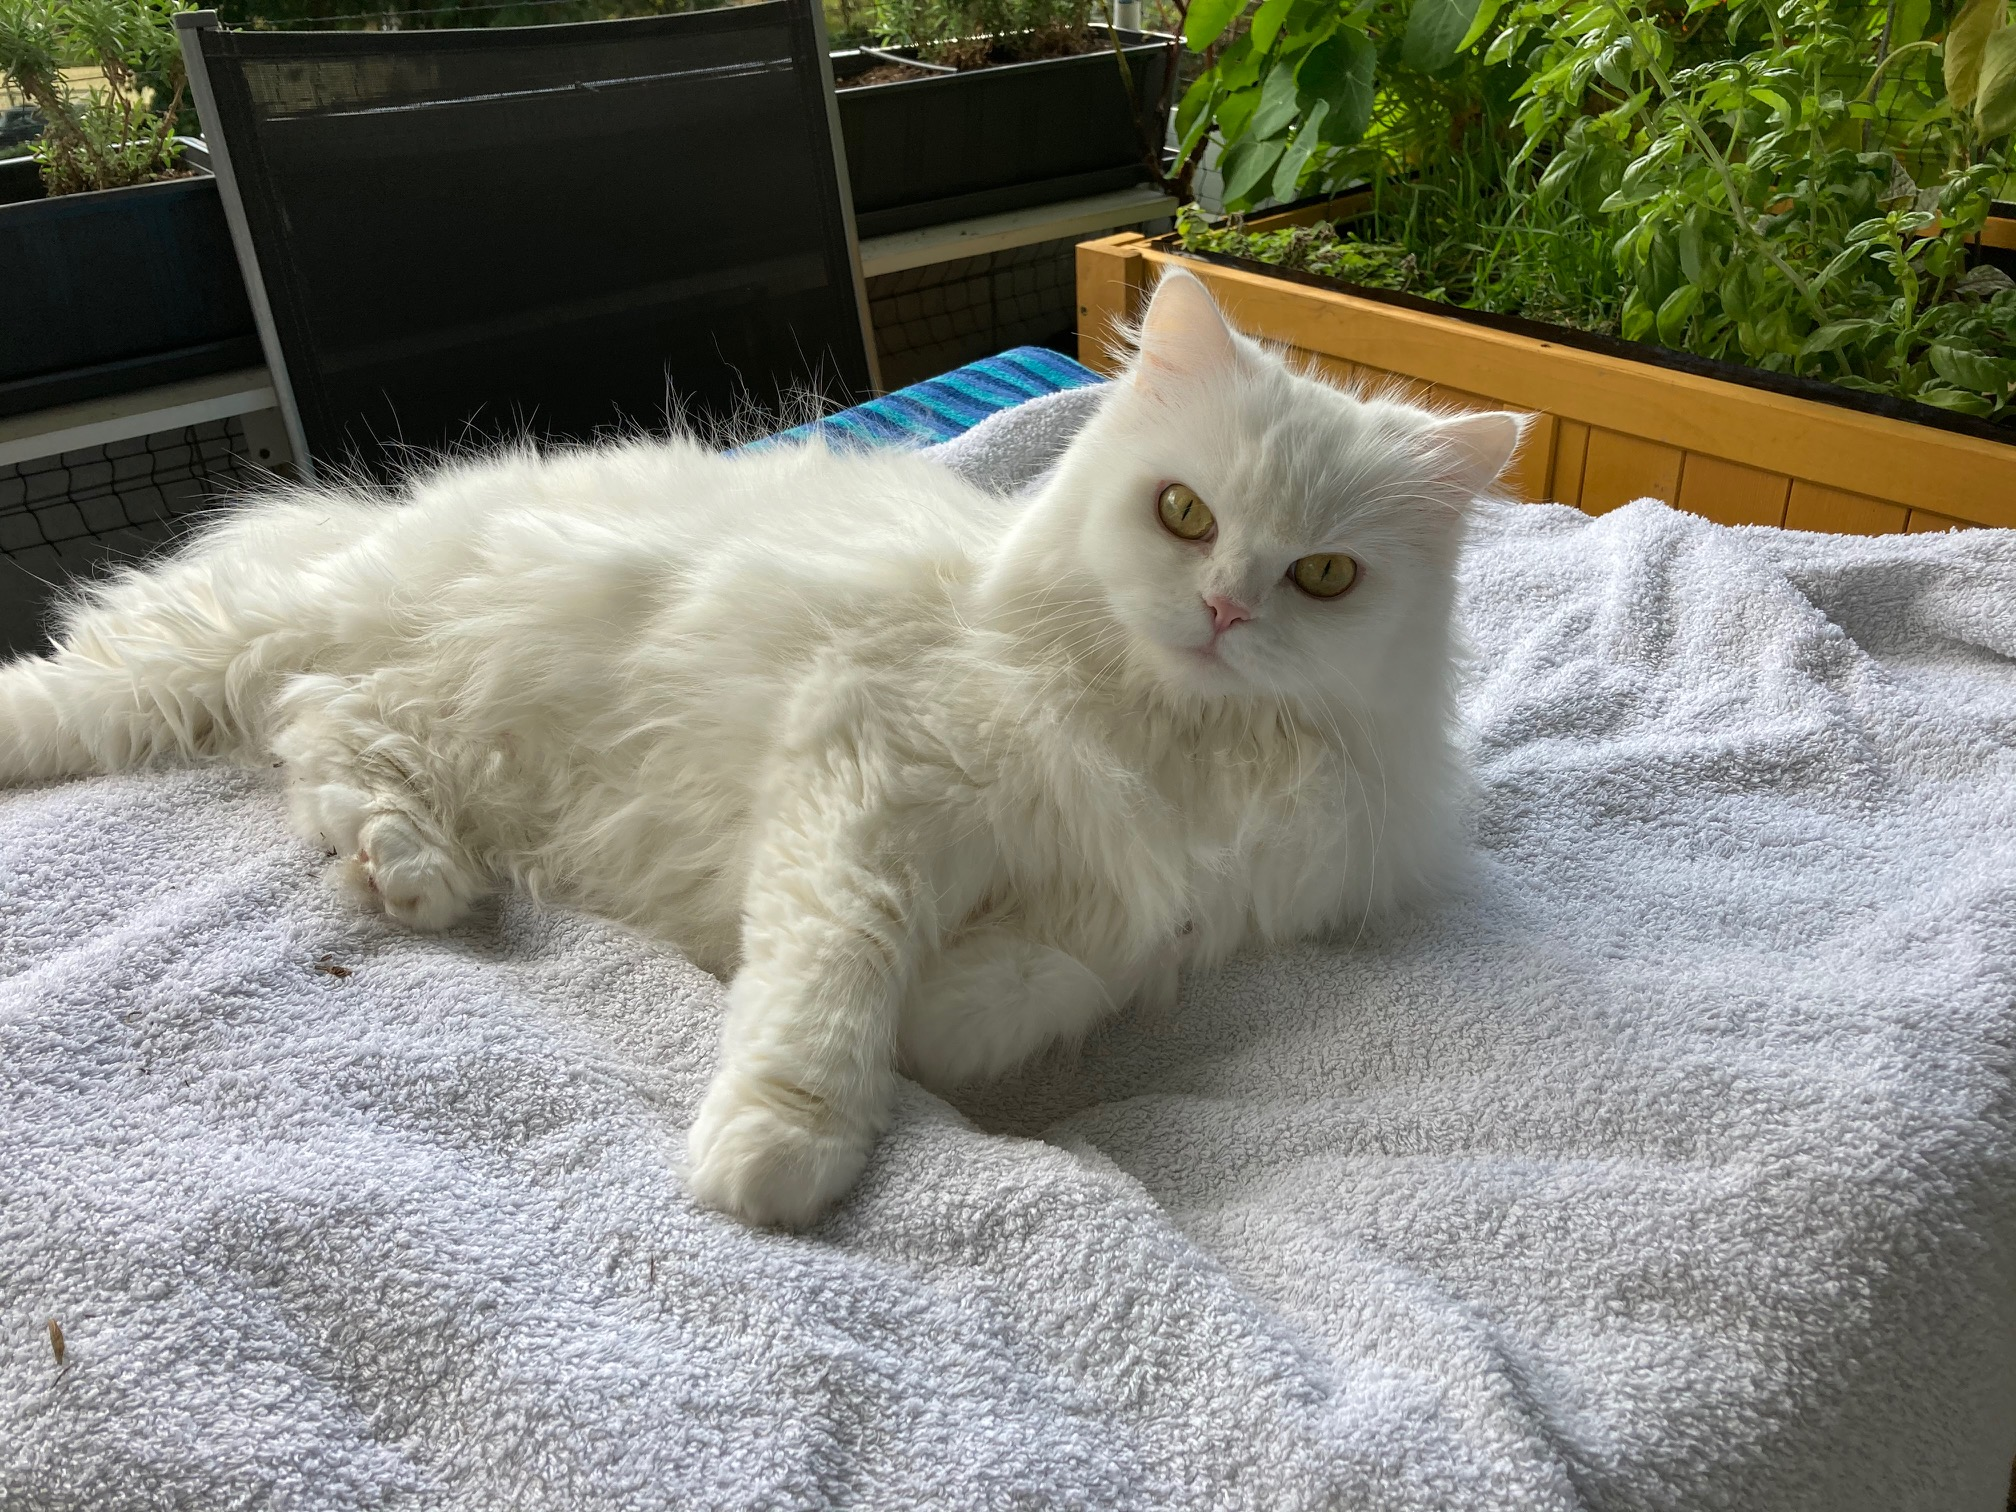
\includegraphics[width=0.8\textwidth]{Bilder/Katze1}
\caption[Kurzversion der caption]{Melli 2, \blindtext}
\end{center}
\end{figure}

\blindtext[10]


\begin{figure}
\begin{center}

\includegraphics[width=0.8\textwidth]{Bilder/miau}
\caption{Melli 3}
\end{center}
\end{figure}

\subsubsection{International}

sdfsdfsd


\blindtext

\section{Analyse} 

\blindtext

\blindtext[10]

\section{Fazit}

\blindtext[10]

Siehe Abbildung \ref{fig:Katze} auf dsadsf sdfsd fsd fsd sdf sdf dsf sdf sdfsd fsd sfsdfsd fsdf df  Seite~\pageref{fig:Katze}

Siehe Abschnitt \ref{sec:Einleitung}

Siehe \prettyref{sec:Einleitung}

Siehe \prettyref{fig:Katze}

\section{Tabellen}
\subsection{Eine einfache Tabelle}
%left, right, center, Absatz mit Breite
\begin{tabular}{lrcp{5cm}}
123 & 456 & 789  & Hallo, ich bin ein Text, der umgebrochen wird nach ca. 5 Zentimetern. \\
24 423 123 & 456 424234 &  32789  & Hallo, ich bin ein Text, der umgebrochen wird nach ca. 5 Zentimetern. \\
\end{tabular}

\subsection{Eine unschöne Tabelle}

\begin{tabular}{|l|r|c|p{5cm}|} \hline
Spalte 1 & Spalte 2  & Spalte 3 & Spalte 4 \\ \hline
123 & 456 & 789  & Hallo, ich bin ein Text, der umgebrochen wird nach ca. 5 Zentimetern. \\ \hline
24 423 123 & 456 424234 &  32789  & Hallo, ich bin ein Text, der umgebrochen wird nach ca. 5 Zentimetern. \\ \hline
\end{tabular} 

\blindtext

\subsection{Eine schöne Tabelle (auch mit booktabs)}

\begin{table}
\caption{Meine schöne Tabelle}\label{tab:erste}
\begin{center}
\begin{tabular}{lrcp{5cm}} \toprule[2pt]
\textbf{Spalte 1} & {\bfseries Spalte 2}  & \textbf{Spalte 3}  & \textbf{Spalte 4}  \\ \cmidrule[1pt](rl){1-4}
123 & 456 & 789  & Hallo, ich bin ein Text, der umgebrochen wird nach ca. 5 Zentimetern. \\ \midrule
24 423 123 & 456 424234 &  32789  & Hallo, ich bin ein Text, der umgebrochen wird nach ca. 5 Zentimetern. \\ \bottomrule[2pt]
\end{tabular} 
\end{center}
\end{table}

\blindtext

\begin{table}
\caption{Meine schöne Tabelle}\label{tab:breite}
\begin{center}
\begin{tabular}{llllllllll} \toprule[2pt]
Spalte 1 	&	Spalte 2	&	Spalte 3	&	Spalte 4	&	Spalte 5	&	Spalte 6	&	Spalte 7	&	Spalte 8	&	Spalte 9	&	Spalte 10	\\ \midrule 
0,638032708	&	0,79774139	&	0,669420835	&	0,130282865	&	0,617404107	&	0,131897273	&	0,160448937	&	0,930336614	&	0,456094857	&	0,882464506	\\
0,430368467	&	0,312526442	&	0,078835549	&	0,186265174	&	0,418099166	&	0,295494638	&	0,235062798	&	0,591799815	&	0,367647474	&	0,318734279	\\
0,460270292	&	0,865033668	&	0,765548665	&	0,277912796	&	0,323193937	&	0,533851539	&	0,678653282	&	0,89105302	&	0,098213808	&	0,714293404	\\
0,454448183	&	0,052457591	&	0,075849422	&	0,315151997	&	0,191617822	&	0,644894383	&	0,322832897	&	0,830696478	&	0,203470593	&	0,194167497	\\
0,644930394	&	0,374040276	&	0,811477249	&	0,561929176	&	0,769846564	&	0,695501883	&	0,140888911	&	0,308050325	&	0,091165056	&	0,683259159	\\
0,052103164	&	0,713379636	&	0,750287656	&	0,078583627	&	0,367974351	&	0,185145035	&	0,622090331	&	0,059947016	&	0,724199449	&	0,970850565	\\
0,793074515	&	0,798765482	&	0,787195706	&	0,580923138	&	0,368506447	&	0,167894819	&	0,55265108	&	0,574037334	&	0,312791086	&	0,110657135	\\
0,270226209	&	0,911089391	&	0,196667473	&	0,818650631	&	0,653616939	&	0,311474239	&	0,054395594	&	0,962807933	&	0,531687051	&	0,41095502	\\
0,046675419	&	0,633715472	&	0,159039988	&	0,62751913	&	0,019329396	&	0,976732473	&	0,010935954	&	0,541956019	&	0,450450328	&	0,700969687	\\
0,477138302	&	0,666779616	&	0,958603602	&	0,746428008	&	0,973369046	&	0,347825874	&	0,663695752	&	0,882285571	&	0,511347685	&	0,865748917	\\
0,841821581	&	0,829187521	&	0,825762327	&	0,650500575	&	0,99314032	&	0,425798748	&	0,67219439	&	0,983308544	&	0,33502473	&	0,189245132	\\
0,628764283	&	0,313479849	&	0,491290001	&	0,63180983	&	0,977592107	&	0,19947654	&	0,542538772	&	0,116343653	&	0,457540675	&	0,608567919	\\
0,243321899	&	0,053950719	&	0,989796288	&	0,937049245	&	0,86013547	&	0,587719616	&	0,892248412	&	0,492928049	&	0,951350427	&	0,836200242	\\
0,598431122	&	0,164907385	&	0,454698909	&	0,623213881	&	0,606691821	&	0,975360578	&	0,750045381	&	0,752994633	&	0,086066313	&	0,974402958	\\
0,46021826	&	0,922561942	&	0,003689839	&	0,447128906	&	0,535373832	&	0,029777978	&	0,35301431	&	0,917187508	&	0,62761049	&	0,008382583	\\
0,041269006	&	0,304680154	&	0,606127874	&	0,61332918	&	0,439920051	&	0,290707773	&	0,595512583	&	0,367226653	&	0,804072552	&	0,614216946	\\
0,137316987	&	0,502349727	&	0,603179459	&	0,742409083	&	0,489874844	&	0,616276892	&	0,944088502	&	0,503252426	&	0,45247528	&	0,318952145	\\
0,717572655	&	0,523894536	&	0,753363854	&	0,126601086	&	0,277323489	&	0,464379265	&	0,261424638	&	0,721794775	&	0,54746453	&	0,568316411	\\
0,747221014	&	0,375369298	&	0,55406433	&	0,206507801	&	0,875896205	&	0,052657457	&	0,939929968	&	0,72876897	&	0,688596567	&	0,957761638	\\
0,136609563	&	0,387307058	&	0,690792381	&	0,348494509	&	0,169671263	&	0,971146736	&	0,09967788	&	0,906900969	&	0,14863983	&	0,965002163	\\
0,349312159	&	0,490830945	&	0,474538058	&	0,628933241	&	0,024893043	&	0,728771809	&	0,508693551	&	0,747369177	&	0,209026177	&	0,684813334	\\ \bottomrule 
\end{tabular} 
\end{center}
\end{table}



\end{document}
